\begin{figure*}[!ht]
    \centering
\begin{minipage}[t]{0.45\textwidth}  % Left block: explanation + plot
    \vspace{0pt}
    \begin{subfigure}[t]{\textwidth}
        \centering
        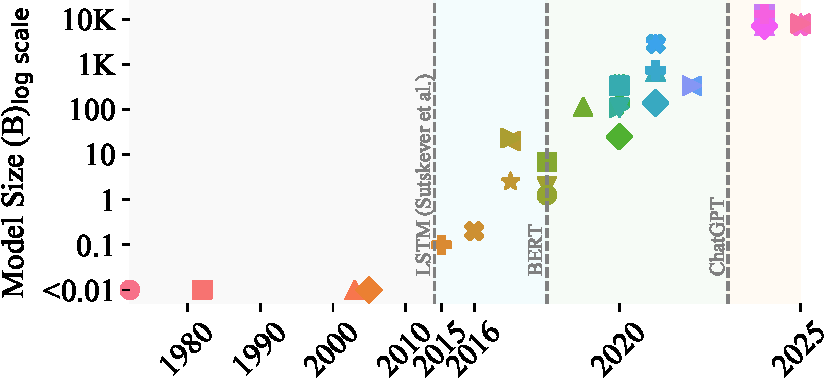
\includegraphics[width=\linewidth]{imgs/model_sizes/model-v.s.-time.crop.pdf}
    \end{subfigure}%
    \small
    \renewcommand{\arraystretch}{1.3}
    \begin{tabular}{l}
   % \bf \textcolor{eraRule}{\rule{8pt}{8pt}} Rule-based \scriptsize up to 2014\\
   \colorbox{eraRule}{\parbox{\linewidth}{\bfseries\textcolor{black}{Rule-based} \scriptsize up to 2014}}\\
   {\it Characteristics}: symbolic, static (\citeyear{woods1972lunar}) \\
   {\it Challenges}: labor-intensive; generalization (\citeyear{warren-pereira-1982-efficient})\\
    % \bf\textcolor{eraSeq2Seq}{\rule{8pt}{8pt}} Seq2Seq \scriptsize 2014\(\sim \)2018 \\
    \colorbox{eraSeq2Seq}{\parbox{\linewidth}{\bfseries\textcolor{black}{Seq2Seq} \scriptsize 2014\(\sim \)2018}}\\
    \begin{tabular}{@{}l@{}}
    {\it Characteristics}: feature engineering (\citeyear{zhong2018seqsql}) \\
   {\it Challenges}: generalization (\citeyear{yu-etal-2018-spider});\\
   \hspace{5em} reasoning \citep{liu2018table}
   \end{tabular}\\
    % \bf\textcolor{eraTransformer}{\rule{8pt}{8pt}} Transformer \scriptsize 2018\(\sim \)2023\\
    \colorbox{eraTransformer}{\parbox{\linewidth}{\bfseries\textcolor{black}{Transformer} \scriptsize 2018\(\sim \)2023}}\\
    \begin{tabular}{@{}l@{}}
    {\it Characteristics}: domain pre-training (\citeyear{yin-etal-2020-tabert}); \\ 
    \hspace{5em}feature engineering (\citeyear{wang-etal-2020-rat})
    \end{tabular}\\
    \begin{tabular}{@{}l@{}}
   {\it Challenges}: generalization (\citeyear{suhr-etal-2020-exploring});\\
   % \hspace{5em}reasoning (\citeyear{xie-etal-2022-unifiedskg});\\
   \hspace{5em}data-intensive (\citeyear{yin-etal-2020-tabert}), etc
   \end{tabular}\\
    % \bf\textcolor{eraLLM}{\rule{8pt}{8pt}} LLM Era \scriptsize 2023 to now\\
    \colorbox{eraLLM}{\parbox{\linewidth}{\bfseries\textcolor{black}{LLM Era} \scriptsize 2023 to now}}\\
    {\it Characteristics}: post-training (\citeyear{zhang-etal-2024-tablellama, yang2025table})\\
    \begin{tabular}{@{}l@{}}
   {\it Challenges}: generalization (\citeyear{deng2025rethinking});\\
   % \\\hspace{5em}complex reasoning (\citeyear{wu2025mmqa});\\
   \hspace{5em}paradox of choice (\citeyear{zhang-etal-2024-tablellama, zhang2024tablellm}), etc \\
   \end{tabular}\\
    \end{tabular}
\end{minipage}
\hfill
  \begin{minipage}[t]{0.52\textwidth}  % Right block: full legend
      \vspace{0pt}
      \centering
        \small
      \renewcommand{\arraystretch}{1.4}
    \begin{tabular}{|>{\raggedright\arraybackslash}p{10em}>{\raggedright\arraybackslash}p{10em}|}
    \hline
    
\includegraphics[scale=0.5]{imgs/model_sizes/lunar.pdf}~LUNAR (\citeyear{woods1972lunar}) & 
\includegraphics[scale=0.5]{imgs/model_sizes/chat_80.pdf}~CHAT-80 (\citeyear{warren-pereira-1982-efficient}) \\

\includegraphics[scale=0.5]{imgs/model_sizes/precise.pdf}~PRECISE (\citeyear{popescu2003towards}) & 
\includegraphics[scale=0.5]{imgs/model_sizes/sumtime.pdf}~SumTime (\citeyear{reiter2005choosing}) \\

\includegraphics[scale=0.5]{imgs/model_sizes/pasupat_&_liang_parser.pdf}~\citet{pasupat-liang-2015-compositional} & 
\includegraphics[scale=0.5]{imgs/model_sizes/neural_enquirer.pdf}~Neural Enquirer (\citeyear{yin-etal-2016-neural}) \\

\includegraphics[scale=0.5]{imgs/model_sizes/neural_programmer.pdf}~Neural Programmer (\citeyear{neelakantan2017learning}) & 
\includegraphics[scale=0.5]{imgs/model_sizes/wiseman.pdf}~\citet{wiseman-etal-2017-challenges} \\

\includegraphics[scale=0.5]{imgs/model_sizes/liu.pdf}~\citet{liu2018table} & 
\includegraphics[scale=0.5]{imgs/model_sizes/seq2sql.pdf}~Seq2SQL (\citeyear{zhong2018seqsql}) \\

\includegraphics[scale=0.5]{imgs/model_sizes/sqlnet.pdf}~SQLNet (\citeyear{xu2018sqlnet}) & 
\includegraphics[scale=0.5]{imgs/model_sizes/typesql.pdf}~TypeSQL (\citeyear{yu-etal-2018-typesql}) \\

\includegraphics[scale=0.5]{imgs/model_sizes/sqlova.pdf}~SQLova (\citeyear{hwang2019comprehensive}) & 
\includegraphics[scale=0.5]{imgs/model_sizes/rat_sql.pdf}~RAT-SQL (\citeyear{wang-etal-2020-rat}) \\

\includegraphics[scale=0.5]{imgs/model_sizes/rat_sql+.pdf}~RAT-SQL+ (\citeyear{wang-etal-2020-rat}) & 
\includegraphics[scale=0.5]{imgs/model_sizes/rat_sql++.pdf}~RAT-SQL++ (\citeyear{wang-etal-2020-rat}) \\
 
\includegraphics[scale=0.5]{imgs/model_sizes/tabert.pdf}~TaBERT (\citeyear{yin-etal-2020-tabert}) &

\includegraphics[scale=0.5]{imgs/model_sizes/table_bert.pdf}~Table-BERT (\citeyear{Chen2020TabFact}) \\

\includegraphics[scale=0.5]{imgs/model_sizes/chen20.pdf}~\citet{chen-etal-2020-hybridqa} &

\includegraphics[scale=0.5]{imgs/model_sizes/tapas.pdf}~TAPAS (\citeyear{herzig-etal-2020-tapas}) \\

\includegraphics[scale=0.5]{imgs/model_sizes/tapas+.pdf}~TAPAS+ (\citeyear{herzig-etal-2020-tapas}) &

\includegraphics[scale=0.5]{imgs/model_sizes/grappa.pdf}~GraPPa (\citeyear{yu2021grappa})\\

\includegraphics[scale=0.5]{imgs/model_sizes/gap.pdf}~GAP (\citeyear{shi2021learning}) &

\includegraphics[scale=0.5]{imgs/model_sizes/chen21.pdf}~\citet{chen2021open}\\

\includegraphics[scale=0.5]{imgs/model_sizes/unifiedskg.pdf}~UnifiedSKG (\citeyear{xie-etal-2022-unifiedskg}) &

\includegraphics[scale=0.5]{imgs/model_sizes/unifiedskg+.pdf}~UnifiedSKG+ (\citeyear{xie-etal-2022-unifiedskg}) \\ 
\includegraphics[scale=0.5]{imgs/model_sizes/picard.pdf}~PICARD (\citeyear{scholak-etal-2021-picard}) &

\includegraphics[scale=0.5]{imgs/model_sizes/tableformer.pdf}~TableFormer (\citeyear{yang-etal-2022-tableformer}) \\
 
\includegraphics[scale=0.5]{imgs/model_sizes/tapax.pdf}~TAPAX (\citeyear{liu2022tapex}) &

\includegraphics[scale=0.5]{imgs/model_sizes/tablellama.pdf}~TableLlama (\citeyear{zhang-etal-2024-tablellama}) \\ 
\includegraphics[scale=0.5]{imgs/model_sizes/tablellm_7b.pdf} TableLLM-7B (\citeyear{zhang2024tablellm}) &

\includegraphics[scale=0.5]{imgs/model_sizes/tablellm_13b.pdf} TableLLM-13B (\citeyear{zhang2024tablellm}) \\ 
\includegraphics[scale=0.5]{imgs/model_sizes/tablegpt_2.pdf} TableGPT-2 (\citeyear{su2024tablegpt2}) &

\includegraphics[scale=0.5]{imgs/model_sizes/tablellava.pdf} TableLlava-7B (\citeyear{zheng-etal-2024-multimodal}) \\

\includegraphics[scale=0.5]{imgs/model_sizes/tablellava_13b.pdf}~TableLlava-13B (\citeyear{zheng-etal-2024-multimodal}) &
% \begin{tabular}{@{}l@{}}
\includegraphics[scale=0.5]{imgs/model_sizes/tablebenchllm_7b.pdf}~TableBenchLLM-7B\\
% \hspace{1em}(\citeyear{wu2025tablebench})
% \end{tabular} \\

\includegraphics[scale=0.5]{imgs/model_sizes/tablebenchllm_7b.pdf}~TableBenchLLM-7B (\citeyear{wu2025tablebench})\\
% \begin{tabular}{@{}l@{}}
\includegraphics[scale=0.5]{imgs/model_sizes/tablebenchllm_8b.pdf}~TableBenchLLM-8B\\
% \hspace{1em}(\citeyear{wu2025tablebench})
% \end{tabular}

\includegraphics[scale=0.5]{imgs/model_sizes/tablebenchllm_8b.pdf}~TableBenchLLM-8B (\citeyear{wu2025tablebench})
&

\includegraphics[scale=0.5]{imgs/model_sizes/tama.pdf}~TAMA (\citeyear{deng2025rethinking}) \\

\includegraphics[scale=0.5]{imgs/model_sizes/tabl_r1.pdf}~Table-R1 (\citeyear{yang2025table}) & \\
\hline
\end{tabular}
\end{minipage}
\caption{Summarization of different eras for table modeling.
We note that the model sizes increase logarithmically with time.
When we enter the LLM era, the community has shifted its attention to instruction tune the foundational models \citep{zhang-etal-2024-tablellama}.
While there are persistent challenges, such as generalization for table models \citep{warren-pereira-1982-efficient, yu-etal-2018-spider, suhr-etal-2020-exploring, deng2025rethinking} across different eras, new challenges emerge. 
\Cref{app-subsec: table-model-history-fig-explain} provides additional details of this plot.
}
\label{fig: table-modeling-history}
\end{figure*}